\makeatletter
\newcommand*{\textoverline}[1]{$\overline{\hbox{#1}}\m@th$}
\makeatother

\subsection{Levelshifters}\label{sec:levelshifter}
To generate sufficient output power thick oxide transitors are used at the output stage. They can generate larger currents compared to thin oxide transistors and support a larger supply voltage. One of the problems with this is that these transistors have a much larger threshold voltage and that the desired gate voltage of the PMOS transistors is entirely out of the range of the thin oxide transistors in the digital front end. Because of this the fast low voltage transitors used in the digital front end cannot generate a large enough $V_{ON}$. Raising the supply voltage of the low voltage transistors in order to increase the output voltage of the mixers will break them. So special care has to be taken when a transition from a low voltage circuit to high voltage thick oxide transistors. To this end a level shifter is designed. In this design special care will be taken to ensure that the voltages across any low voltage transistor will not exceed 1.2V, so they will not break. On the output side it has to be able to drive very large transistors. The driven NMOS transistors will have to be supplied with a voltage of 0V(off) to 2V(on) and the driven PMOS transistors with a voltage of 5V(off) to 3V(on). 
In~\cite{powerdac} a design for the levelshifter was proposed, but they were not able to integrate it with the rest of their design. Some other designs looked at are proposed in~\cite{koo2005new} and~\cite{hass2000level}. In this paper the design from~\cite{powerdac} is chosen, because the others did not look as promising and are intended for different scenarios compared to the situation in this paper. Designing the levelshifter caused some major problems. First the cadence models originally used have have an unrealistically high threshold voltage of 1.5V, this makes it difficult to drive them with the thin oxide transistors. In order to create a functioning simulation this was changed to a more realistic threshold voltage of 0.7V. This gives a larger $V_{ON}$, making the transistors conduct more current for a smaller size. This is necessary, because the transistors being driven by the level shifter will be very large. Therefore a large driving current must be supplied by the levelshifter. Another problem that took a lot of time to solve was that the models break down when a 5V $V_{DS}$ is used as  a test load transistor. It caused such a large current into the gate that the rest of the levelshifter broke down, without clear indication as to why this happened. Using a $V_{DS}$ of 2.5V for the test loading transistor, which is also more like the final implemenation, solved this. 
The design of the levelshifter started with the design of the PMOS driver, which should have an output voltage of 3(off) to 5V(on). As a starting point the design from~\cite{powerdac} was used, it is shown on the right in Fig.~\ref{fig:schematic_levelshifter}. In this design the thick oxide transistors M3 and M4 serve to protect the thin oxide transistors M5 and M6 from too high voltages. M1 and M2 form a current sensing circuit that charge the output node and each other's gates when switching. Their most important parameter is their width, the larger they are the quicker they charge the output. But a larger M1 and M2 also means that the M3-6 need to be larger to discharges the nodes. Since M2 must drive both M1 and the load it will be bigger than M1. The next most important parameters are the lengths of M3 and M4 and widths of M5 and M6. together they determine the speed at which the output nodes are discharged and the voltage level of the output nodes when M3 and M5 or M4 and M6 are active. The circuit operates as follows. Assume initially VIN is high and \textoverline{VIN} is low. Node \textoverline{VOUT} will be pulled low by the left branch and the right branch will not conduct any current. Then \textoverline{VOUT} is pulled towards 3V and M2 will start conducting and charging node VOUT towards 5V. This will make M1 stop conducting current, causing \textoverline{VOUT} to be pulled even closer to 3V. In this way M2 and M1 drive each other's gate and amplify each other, enabling fast switching. When everything is settled VOUT should be near 5V and \textoverline{VOUT} near 3V. When the input switches (VIN goes low and \textoverline{VIN} goes high) the process is reversed. Node VOUT will be pulled towards 3V and no current will be conducted by the left branch, enabling \textoverline{VOUT} to be driven towards 5V. Again, M1 and M2 will amplify this process and switch VOUT from 5V to 3V and vice versa for \textoverline{VOUT}.
To drive the NMOS transistors of the DAC's output current sources an extra stage is added to the level shifter. Because the threshold voltage is lowered to 0.7V the VIN signal can weakly drive M8 to pull the output to 0V when VIN is high. VOUT is high then, so M7 will not conduct current. When VIN is low, VOUT is near 3V and M7 will conduct current, pulling VOUT\_NMOS to 2V. For the NMOS driver important parameters were the length of M7, which largely determines the maximum voltage of the output, and the widths of both M7 and M8, which mostly detemine the speed at which it can switch the load. For both the PMOS and NMOS drivers VBIAS determines the maximum $V_{DS}$ of M5 and M6 and is set to make sure $V_{DS}$ has a maximum value of 1.2V.
\begin{figure}[h]
 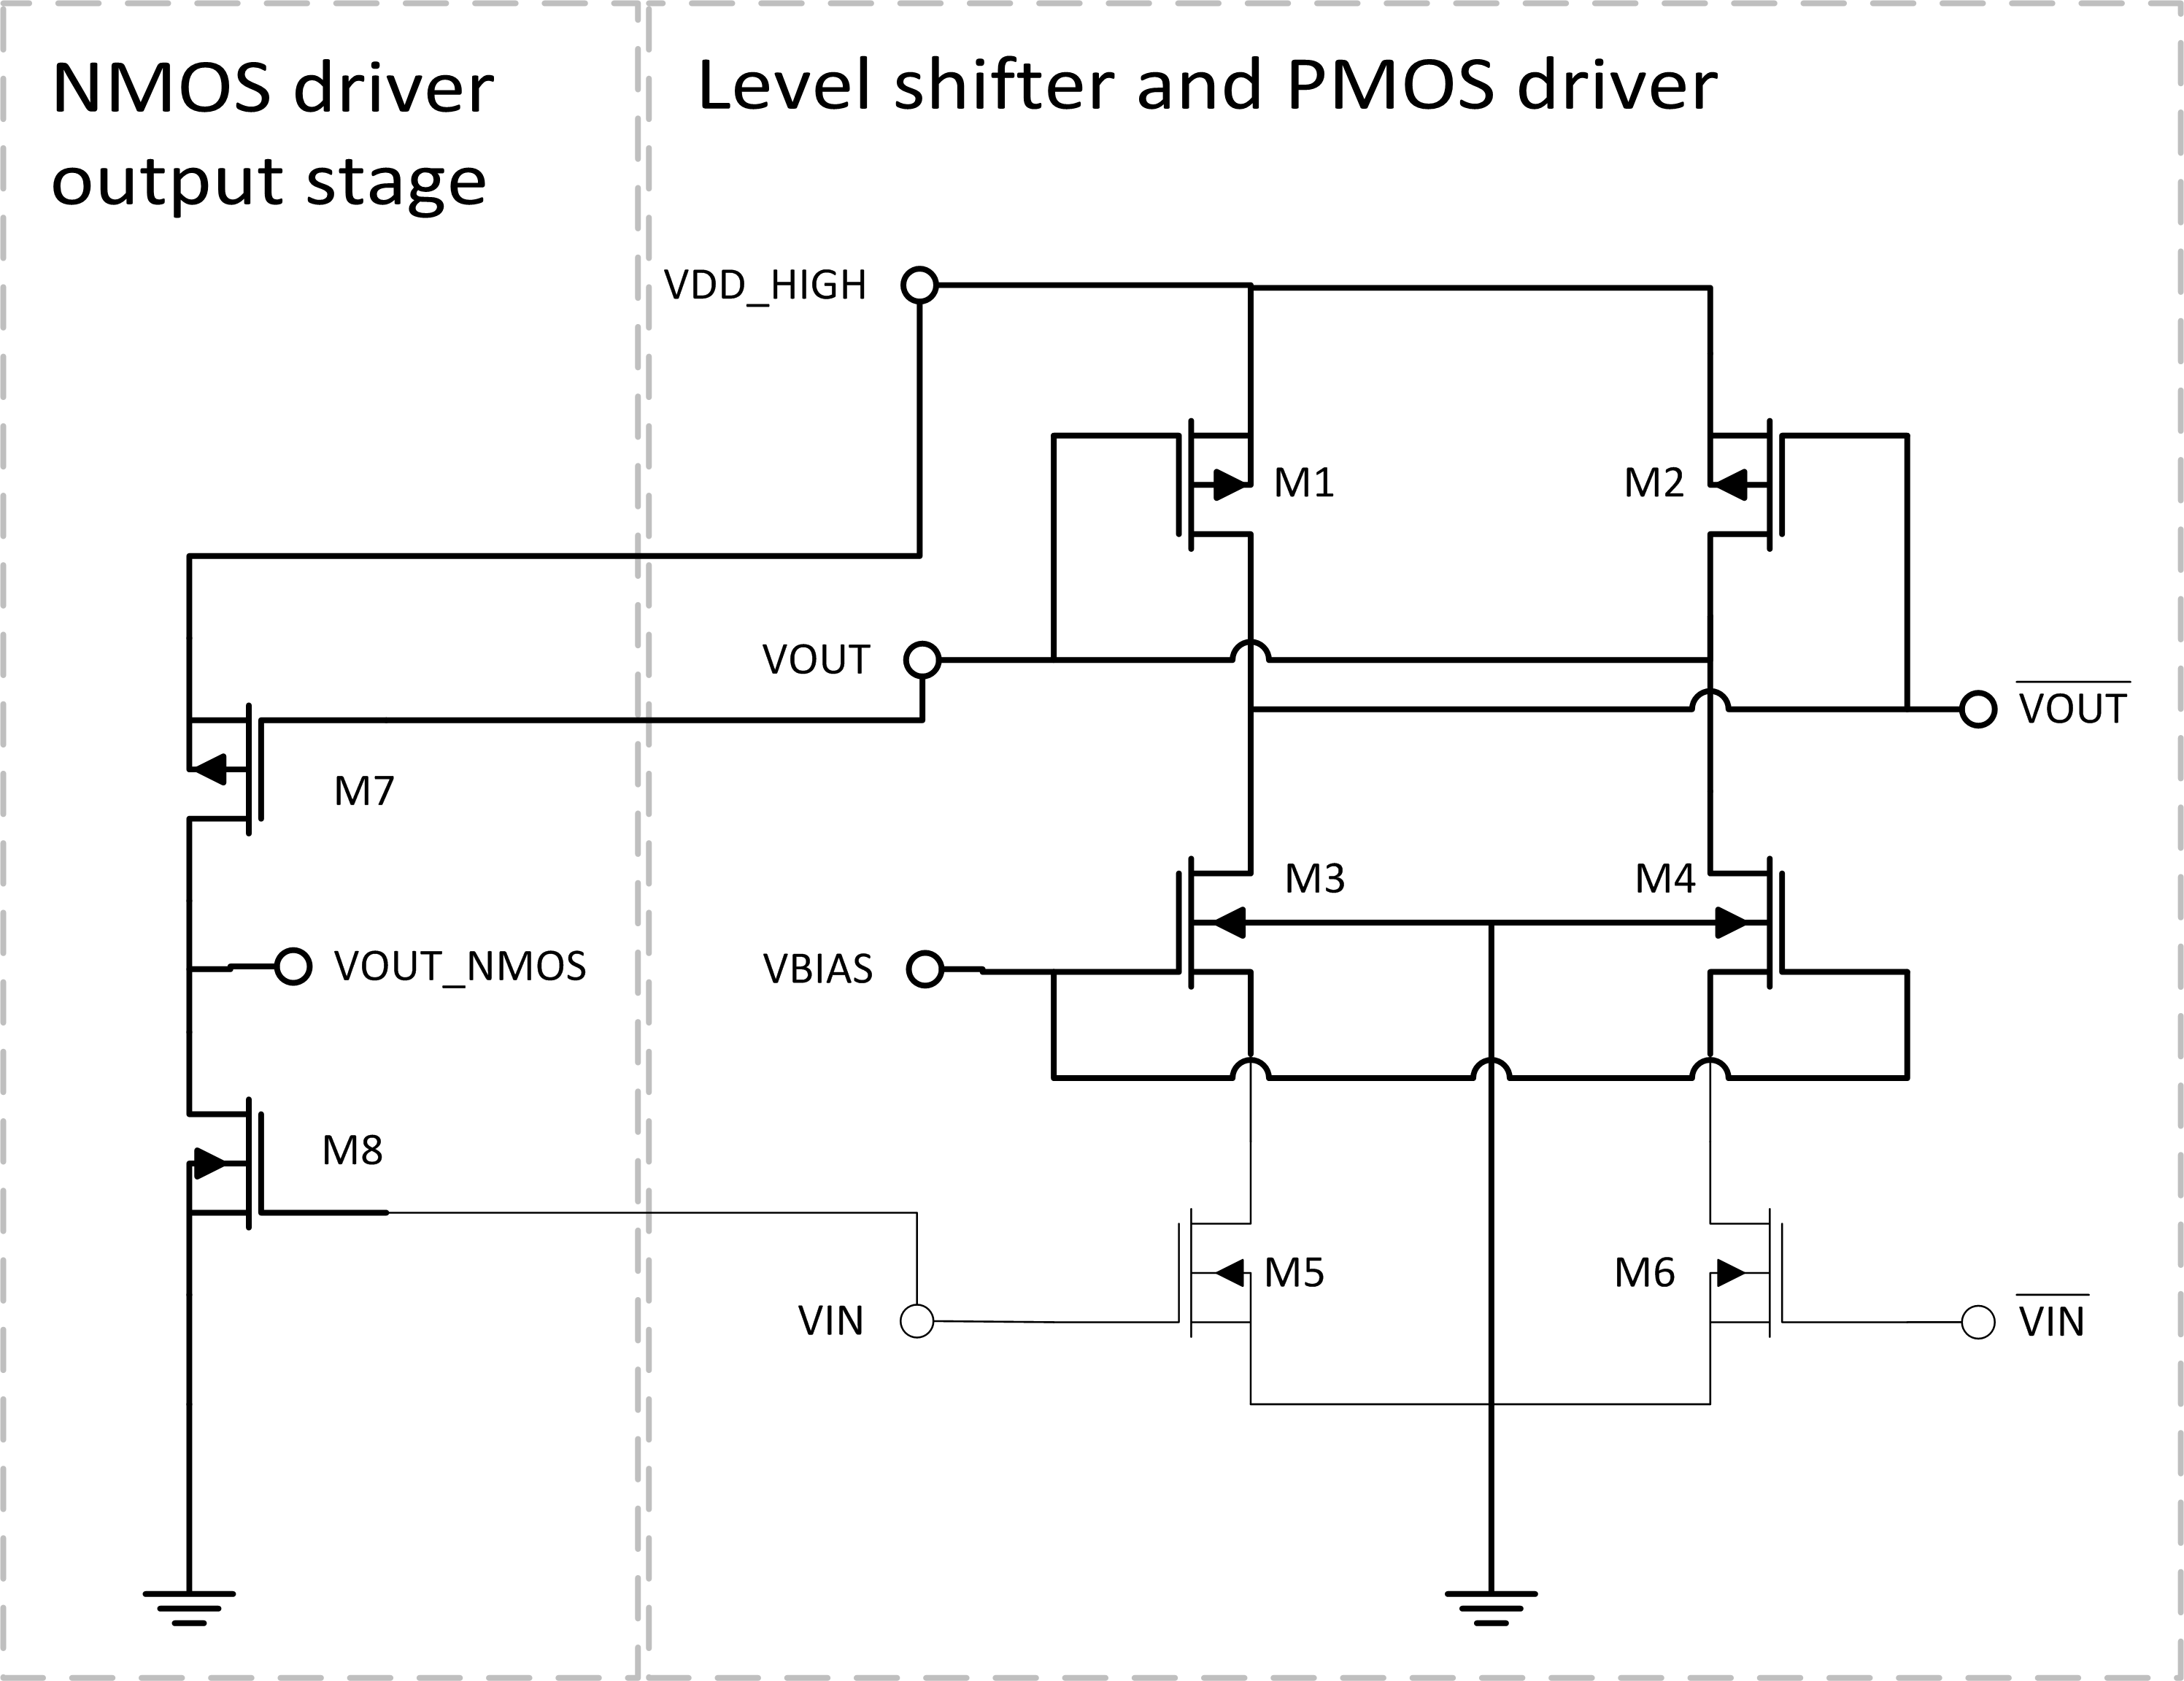
\includegraphics[width=0.5\textwidth]{levelshifter_schematic}
 \caption{Schematics of the levelshifter, thick wires indicate a high voltage regime and thin lines the low voltage transistors. On the right the up-shifting PMOS driver is shown. Its output VOUT can drive a PMOS transistor. The NMOS driver's layout is the same with an extra stage added on the left side. The node VOUT\_NMOS can drive a NMOS transistor.}
 \label{fig:schematic_levelshifter}
\end{figure}
The final sizes of transistors in the PMOS and NMOS driving levelshifters are listed in Appendix~\ref{sec:appendix} in Tables~\ref{Tab:Levelshifter_PMOS_sizes} and~\ref{Tab:Levelshifter_NMOS_sizes} respectively. How these sizes have been determines is discussed next. Both M1 and M2 should have a $V_{DS}$ as low as possible, so their length is set to the minimum of 200n. Their width determines how fast they can charge the load and each other and is determined using the sweep in Fig.~\ref{fig:levelshifter_sweep}. The load of the PMOS driver is a PMOS transistor of size 200nm by 60$\mu$m, approximately the size of the current source PMOS transistors. It shows that a larger width is faster, but at some point increasing its size loses effect. Using this sweep it is chosen to be 60$\mu$m to allow for a carger loading capacitance. After this the size of M1 was determined in a similar fashion. The output voltage level is most depended on the combination of the lengths of M3 and M4 and widths of M5 and M6, these are determined together by sweeping over both parameters and chosing the value combination that comes closest to 3V. They influence the switching speed, but this variation is small and it is more important that the voltage does not drop below 3V to keep the load PMOS in saturation. Finally the other parameters are fine tuned.
\begin{figure}[h]
 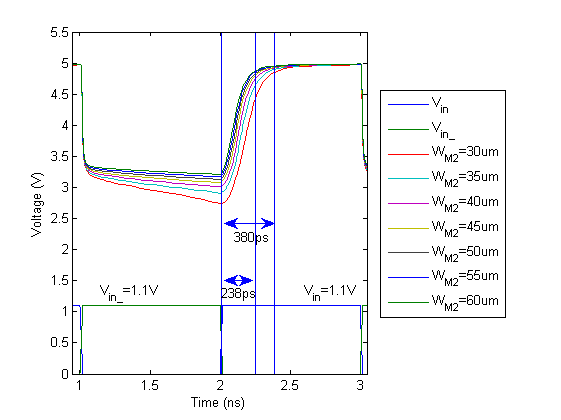
\includegraphics[width=0.5\textwidth]{lvlshift_sweep_wP2.png}
 \caption{Parameter sweep of the width of M2, with a thick oxide PMOS transistor of 200nm by 60$\mu$m as load.}
 \label{fig:levelshifter_sweep}
\end{figure}
To determine the sizes of the transistors of the NMOS driver the PMOS driver is used a starting point. This works since it is still only one PMOS transistor being driven by the original circuit, which shows little variation for different load sizes. So initial tuning ofM7 will have little effect on the behaviour of the original circuit. The maximum output voltage level is determined mostly by the dimensions of M7, which are chosen by a combined sweep. The dimensions of M8 determine how fast the output voltage drops. The length is set to the minimum possible value and the width determined using a standard sweep. A too large transistor cannot be driven by the digital front end and too small will not be able to drive the output current sources. The width is chosen such that a larger width does not change the output a lot.

A final aspect of interest is the power consumption of the levelshifter. This is determined mostly by the current necessary for driving the load transistor. The gates of the load are both charged and discharged via the levelshifter, causing most of the powerconsumption. But also the levelshifter's transistors are relatively large and cost significant power to switch. Simulation results are not available yet. 